\subsection{Experimental Evaluation}
\label{sec:evaluation}
The F-zkNN probabilistic classifier was evaluated on future water consumption forecasting and the extraction of useful knowledge from consumption time-series data, collected in a city scale by smart water meters in Switzerland and Spain. 

\subsubsection{Experimental Setup}
\label{subsec:expsetup}
The experimental evaluation was conducted on a distributed and parallel environment. The setup includes a system with 4 CPUs each containing 8 cores clocked at 2.13GHz, 256GB RAM and a total storage space of 900GB. The total parallel capability of the system reaches the 64 threads. The F-zkNN algorithm is executed by using 16 task managers with 8192MB heap size each.

We firstly experimented on a real-world dataset coming from Switzerland (Switzerland dataset for short). It included shower events from 77 households, each containing an identifier, a timestamp, a smart water meter measurement calculated in litres, the average temperature and demographic information. This information was related to the age, income, number of males or females and total number of household members. This dataset counts 5795 records. To increase its volume and assess the classifier's prediction efficiency, we used the \textit{BigDataBench}\footnote{http://prof.ict.ac.cn/BigDataBench/}, which is a big data generator. We created various synthetic dataset sizes, scaling from 50K records to 15M records.

In the next step, we experimented on large-scale real-world smart water meter data coming from Spain (Spain dataset for short). The water consumption data were formed in hourly time-series coming from 1000 households and covering a time interval of a whole year, i.e. from July 2013 to June 2014. The records included an identifier, a timestamp and a smart water meter measurement calculated in litres. This dataset was constituted by 8.7M records.

The optimal value of the $k$ parameter for the F-zkNN probabilistic classifier was determined through an experimental investigation. The best choice in our context and datasets was proven to be the value of 15. To overcome the lost precision due to the sampling stage, two shifts were adequate on the datasets.

\subsubsection{Feature Selection}
\label{subsec:feautures}
Water consumption time-series pose several challenges on applying machine learning algorithms for classification and forecasting. Thus, proper features that represent and correlate different aspects of the data need to be defined in order to also draw useful conclusions about the determinants that affect water consumption.

Regarding the Switzerland dataset, which included demographic information, we used a dataset of increased volume generated by the BigDataBench (15M records). We took into consideration the sex, the age and the income of the person that generated the shower event. We assessed the classifier by using binary classification for these three features. The sex prediction was made by using the showers for which we knew whether the person was male or female, i.e. households with only one, or of the same sex inhabitants. The age prediction involved the determination of whether the person that generates the shower event is of age less than 35 years, or not. Finally, the income prediction involved the identification of whether the person that takes the shower has income less than 3000 CHF or not. 

Concerning the Spain dataset (8.7M records), we took into consideration several temporal and seasonal features, expressed by different time intervals, which affect the water usage and demand, i.e. the daily time-zone (i.e. [09:00-17:00), [17:00-21:00), etc.), the hour, the weekday, the month and the season. According to each household's mean monthly water consumption in litres, the customers' water usage was categorized from ``very environmental friendly'', to ``significantly spendthrift''. By averaging the hourly water consumption and determining the highest and lowest value, five equally ranged, demand classes were determined, i.e. ``minimum'' ($<$6 litres), ``low'' ($\ge$6 and $<$15 litres), ``normal'' ($\ge$15 and $<$23 litres), ``high'' ($\ge$23 and $<$40 litres) and ``maximum'' ($\ge$40 litres). Besides, we integrated weather conditions via the \textit{Weather Underground} API\footnote{http://www.wunderground.com/}. The integrated weather conditions included the hourly temperature, humidity, and continuous rainfall or heat. 

\subsubsection{Quantitative Evaluation}
\label{subsec:fzknn_results}
The F-zkNN probabilistic classifier was evaluated in the direction of prediction accuracy and useful knowledge extraction, for both datasets. The algorithm was evaluated by forecasting water consumption classes for specific time intervals and also by drawing useful conclusions related with user characteristics (i.e. sex, age and income). Due to space shortage, the figures show results either for forecasting or for knowledge extraction.

The classifier regarding the forecasting was evaluated over the Spain dataset and the prediction of next day's hourly consumption of one or more households for a given time interval. Figure~\ref{fig:example} shows a visualization of the classifier's output. The hourly water consumption characteristics are distributed into classes. The bars indicate the hourly probability of one or more households water consumption to be characterised by each demand class. 

\begin{figure}[htbp]
	\centering
	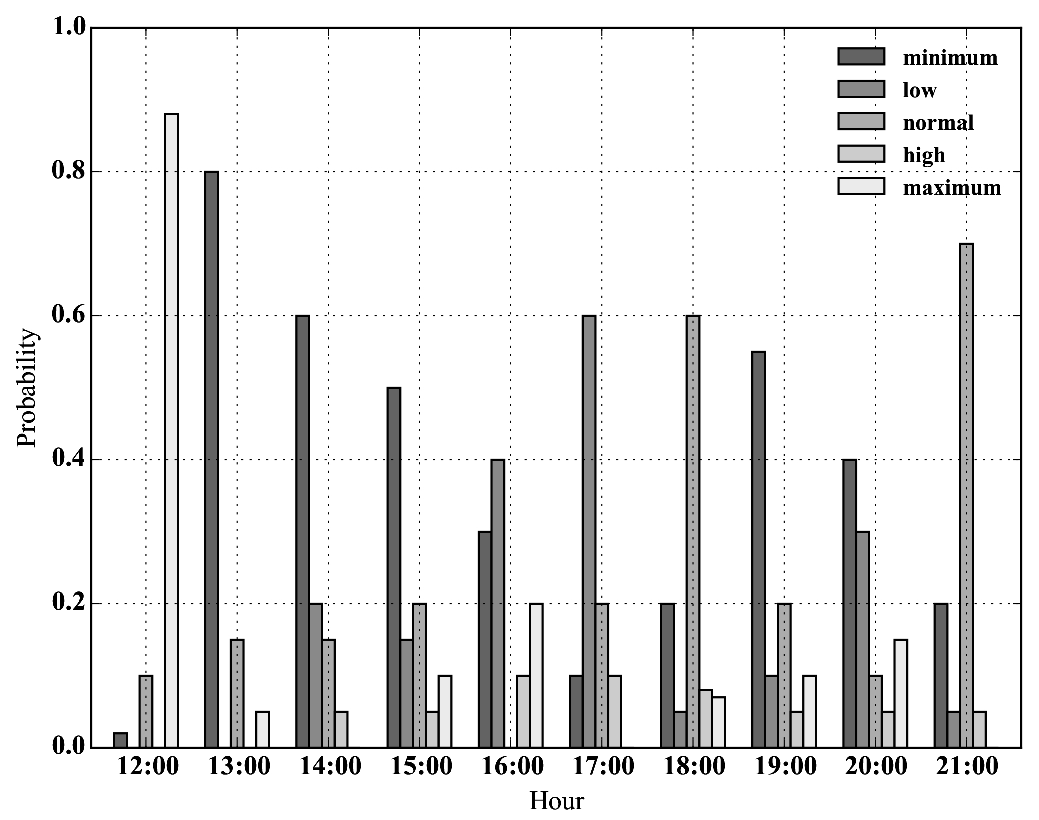
\includegraphics[width=0.5\textwidth]{figures/example.pdf}
	\caption{Hourly forecasting of each consumption class.}
	\label{fig:example}
\end{figure}

Regarding the Switzerland dataset, we used the ten-fold \textit{cross-validation} approach in order to assess useful knowledge extraction. To achieve that, we iteratively split each dataset into ten equal parts and executed the algorithm the same number of times, using a different subset as training set ($R$) and the rest of the sets, unified, as testing set ($S$). The classifier achieved a prediction precision of 78.6\%, 64.7\% and 61.5\% for sex, age and income, as illustrated in Figure~\ref{fig:amphiro_precision}. The results provided us with useful insights concerning water consumption determinants. An important determinant of shower water demand is hair length. Females who have longer hair consume more water. The wrong sex predictions (i.e. 21.4\% out of 100.0\%), is due to the variable hair length of each sex. Moreover, age and income are less important determinants than sex, as people consume water for their daily needs, regardless their age and income. People with a decent income can afford having more expenses regarding their water consumption. Similarly, younger people are well informed about the environmental sustainability, resulting in less wasteful showers.

\begin{figure}[htbp]
	\centering
	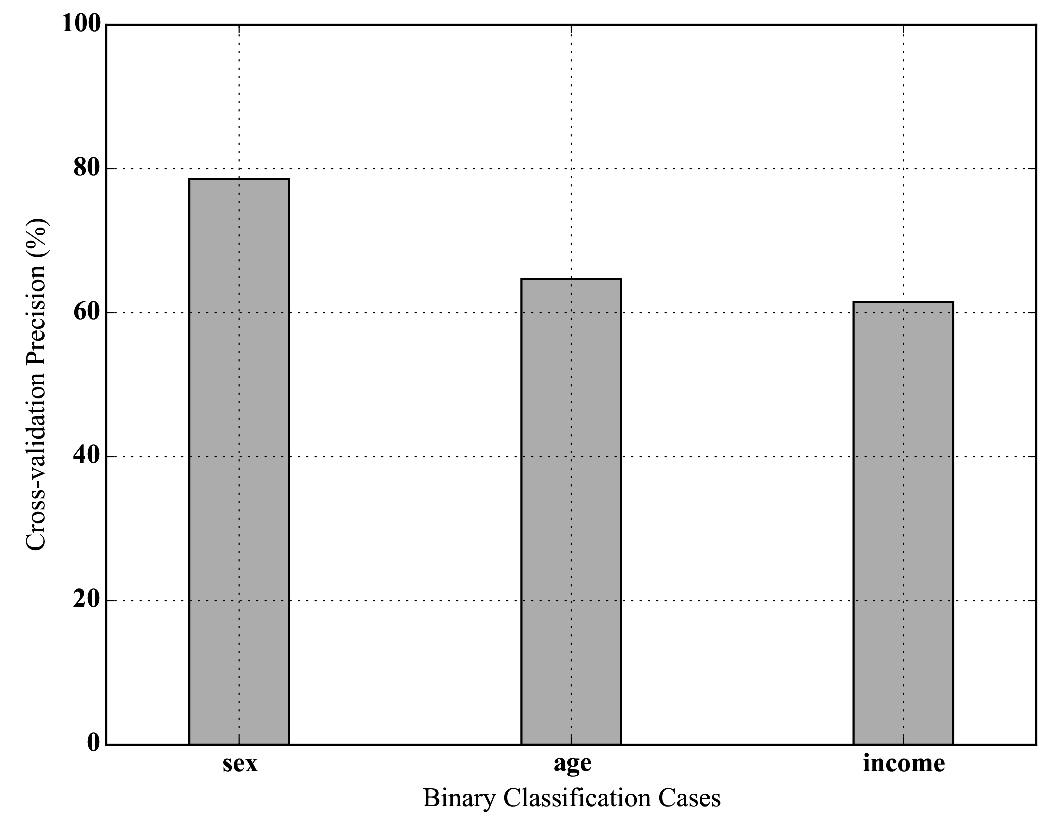
\includegraphics[width=0.5\textwidth]{figures/amphiro.pdf}
	\caption{Prediction precision for sex, age and income.}
	\label{fig:amphiro_precision}
\end{figure}



%Moreover, the classifier's forecasting efficiency was evaluated by computing its precision in retrieving the correct class for each element on different dataset sizes, by splitting the set of 8.7M records into subsets and performing ten-fold cross-validation on each subset. 
%
%Figure~\ref{fig:precision} shows how the F-zkNN probabilistic classifier performs if executed by applying one or two shifts. The advantage of using shifts is apparent, as the algorithm performs 1-2\% better in all dataset sizes. It is noticeable that as the training set's ($S$) size increases, the precision is improved, due to the existence of more elements that can be even closer to the ones that constitute the query. For the full dataset, the precision converges at 68\%. It is worth pointing out that the drop in precision from the 1.7M to the 2.7M dataset is due to over-fitting in one of the cross-validation folds, caused by the insertion of new items. This is apparently overcome on the 3.7M dataset, where the precision rises dramatically. 
%
%\begin{figure}[htbp]
%	\vspace{-3mm}
%	\centering
%	\includegraphics[width=\columnwidth]{images/precision.pdf}
%	\vspace{-3mm}
%	\caption{Prediction precision for water consumption.}
%	\label{fig:precision}
%	\vspace{1mm}
%\end{figure}

 





